\textbf{Icon-Files}\\
Für die Anwendung wird zum einen eine Icon-Datei für die Dialoge und Fenster benötigt. Hierzu ist eine .png-Bilddatei erstellt worden, da das Qt-Framework dieses Format für alle Icons innerhalb der Anwendung unterstützt.\\
Für ein Icon für die exe-Datei kann jedoch keine .png-Bilddatei verwendet werden, sondern es muss eine .ico-Datei erstellt werden. Als Programm zum Erstellen der ico-Datei ist Gimp gemäß \cite{CreateICO} verwendet worden. Das Tutorial beschreibt den exakten Weg zum Erstellen aller Bildformate für Windows. Die ico-Datei muss anschließend im Qt-Projekt konfiguriert werden. \cite{SetICO} benennt die notwendigen Schritte: Im Projekt-Ordner muss eine .rc-Datei mit dem Inhalt "`IDI\_ICON1 ICON    DISCARDABLE "nameOfIco.ico""' angelegt werden. Zum Abschluss muss in der .pro-Datei des Projektes die Zeile "`RC\_FILE = myapp.rc"' eingefügt werden.\bigskip \\

\textbf{BookModel}\\
Das BookModel, abgleitet von QAbstractTableModel, enthält alle Buchdaten. Die Daten werden aus der Datenbank gelesen und zeilenweise im Model abgespeichert. Folgende Methoden sind reimplementiert:
\begin{description}
	\item[ ] explicit BookModel(BookTable *table, LendingTable *ltable, QObject *parent = nullptr)\\
	Initialisiert das Model mit den notwendigen Informationen, dies sind ein Verweis auf die BookTable und LendingTable der Datenbank-API sowie ein optionaler parent.
  \item[ ] \~{}BookModel()\\
	Zerstört das Model und löscht alle Daten in ihm aus dem Speicher.
  \item[ ] QVariant headerData(int section, Qt::Orientation orientation, int role = Qt::DisplayRole) const override\\
	Liefert die Headerinformationen zurück. Diese sind: Titel, Untertitel, ISBN, Jahrgangsstufe, Fach und verfügbare Anzahl eines Buches.
  \item[ ] int rowCount(const QModelIndex \&parent = QModelIndex()) const override//
	Liefert die Anzahl der Zeilen, gleich die Anzahl der Bücher im Model.
  \item[ ] int columnCount(const QModelIndex \&parent = QModelIndex()) const override\\
	Das Model besitzt sechs Spalten, diese wird von dieser Methode zurückgegeben.
  \item[ ] QVariant data(const QModelIndex \&index, int role = Qt::DisplayRole) const override\\
	Liefert die Information pro Zeile und Spalte (dem Index) pro Role zurück. Diese Informationen entsprechen dem jeweiligen Header.
  \item[ ] bool removeRows(int row, int count, const QModelIndex \&parent = QModelIndex()) override\\
	Löscht das Buch aus der Datenbank und dem Model. Vorab wird überprüft, ob das Buch noch ausgeliehen ist, indem Fall darf und wird das Buch nicht gelöscht aber eine Warnung angezeigt.
  \item[ ] void reset()\\
	Setzt das Model zurück.
  \item[ ] void search(QString searchstring)\\
  Filtert anhand des searchstring nach passenden Büchern. Alle nicht passenden Bücher werden aus dem Model entfernt.
  \item[ ] BookTable::BookRow* getRow(QModelIndex row)\\
	Mit dieser Methode kann der zu einer Zeile (row) gehörende Bucheintrag zurückgegeben werden. Diese Methode wird benötigt, um eine Buchzeile in einer Maske bearbeiten zu können.
  \item[ ] void updateRow(int row)\\
	Weist die View des Models an, die entsprechende Zeile neu zu laden. Sie wird ebenfalls benötigt, um eine Buchzeile in einer Maske bearbeiten zu können.
  \item[ ] void addRow(BookTable::BookRow * newRow)\\
	Durch den Aufruf dieser Methode kann dem Model eine neue Buchzeile (newRow) hinzugefügt werden.	
\end{description}

\textbf{BookWidget}\\
Das BookWidget, siehe Abbildung \ref{fig:BookWidget}, kann in ein Fenster eingebettet werden. Es besitzt ein Objekt der Klasse BookModel, um die darin enthaltenen Bücher anzuzeigen. BookWidget ist von QWidget abgeleitet. Seine Methoden sind:
\begin{description}
	\item[ ] explicit BookWidget(Dataset *set, QWidget *parent = 0)\\
	Konstruiert eine neue Instanz von BookWidget, dazu muss ihm das Dataset und optional ein parent übergeben werden. 
  \item[ ] \~{}BookWidget()\\
	Zerstört das Objekt und gibt den Speicherplatz wieder frei.
	\item[ ] Signal: void closewidget()\\
	Dieses Signal wird emittiert, wenn das BookWidget verworfen werden soll.
\end{description}
Das BookWidget erlaubt es, Bücher anzuzeigen, diese zu filtern, Bücher hinzuzufügen und zu löschen. Außerdem können Bücher mittels einer Maske bearbeitet werden.
\begin{figure}[htb]
	\centering
		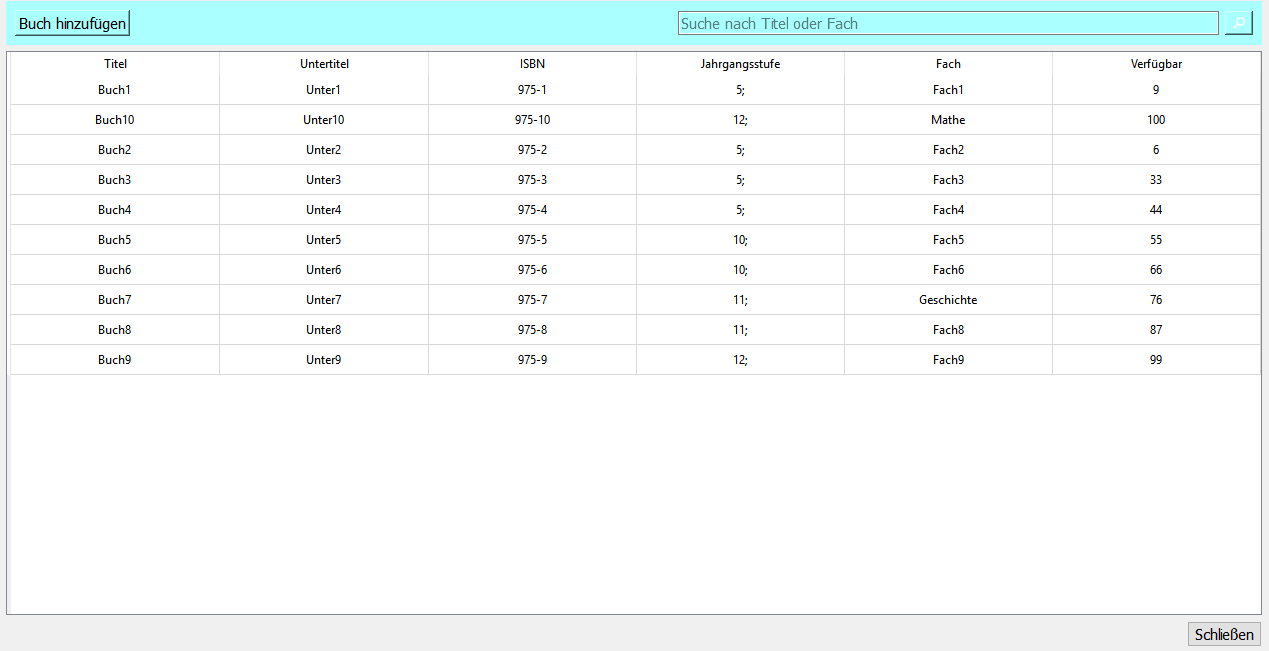
\includegraphics[width=0.70\textwidth]{figures/BookWidget.PNG}
	\caption{BookWidget}
	\label{fig:BookWidget}
\end{figure}
 \bigskip \\

\textbf{BookMask}\\
Die BookMask-Klasse beinhaltet den Dialog zur Bearbeitung und Neuanlage von Büchern. Er ist in Abbildung \ref{fig:BookMask} abgebildet. Ihre Basisklasse ist QDialog. Die öffentlichen Methoden sind:
\begin{description}
	\item[ ] explicit BookMask(BookTable *table, QWidget *parent = 0)\\
	Erzeugt die Büchermaske. Das Objekt benötigt einen Pointer auf die BookTable des Dataset und optional einen parent für den Dialog.
  \item[ ] \~{}BookMask()\\
	Zerstört das Objekt und gibt den Speicher wieder frei.	
  \item[ ] BookTable::BookRow* getInsertedBookRow()\\
	Liefert die neu erstellte Zeile zurück.
  \item[ ] void setBookRow(BookTable::BookRow* row)\\
	Übergibt eine Bücherzeile an die Büchermaske zur Bearbeitung und Anzeige.
\end{description}
\begin{figure}[htb]
	\centering
		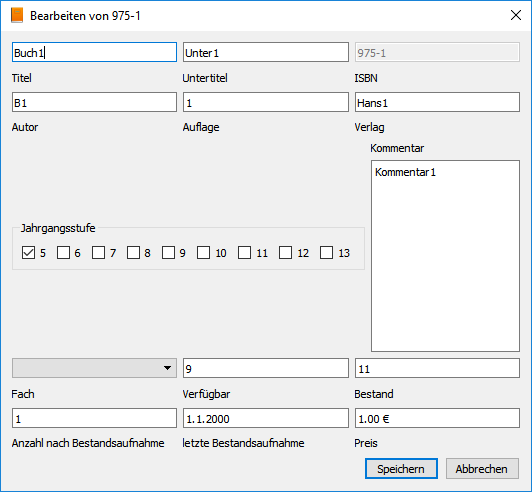
\includegraphics[width=0.60\textwidth]{figures/BookMask.png}
	\caption{Büchermaske}
	\label{fig:BookMask}
\end{figure}

\textbf{DamageDialog}\\
Der DamageDialog dient zur Abfrage, ob ein Buch beschädigt ist. Ein Beispiel des Dialogs ist in Abbildung \ref{fig:DamageDialog} dargestellt. Der Dialog erbt von QDialog, weitere Methoden sind:
\begin{description}
	\item[ ] explicit DamageDialog(QString forename, QString surname, QString booktitle, QWidget *parent = 0)\\
	Erzeugt ein Objekt von DamageDialog unter Angabe eines Vornamens, eines Nachnahmens und eines Buchtitels. Diese Informationen werden im Dialog angezeigt.
	\item[ ] \~{}DamageDialog()\\
	Zerstört das Objekt und gibt den Speicherplatz frei.	
  \item[ ] QString getDamage()\\
	Liefert den eingetragenen Schaden zurück. Wird kein Schaden vergeben, so wird ein leerer String zurückgegeben.
\end{description}
\begin{figure}[htb]
	\centering
		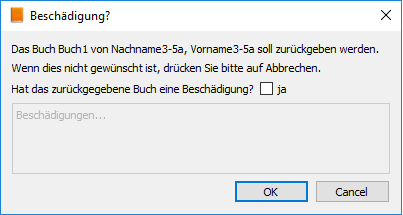
\includegraphics[width=0.60\textwidth]{figures/DamageDialog.png}
	\caption{DamageDialog}
	\label{fig:DamageDialog}
\end{figure} 

\textbf{DamagesWidget}\\
Das DamagesWidget zeigt alle Rückgaben des jeweiligen Schülers in Form eines Baumes an. Durch den "`Begleichen"'-Button wird der Schaden aus der Rückgabe entfernt. Das Widget ist in Abbildung \ref{fig:DamagesWidget} abgebildet.
\begin{description}
	\item[ ] explicit DamagesWidget(Dataset* set, QWidget *parent = 0)\\
	Erzeugt ein neues Objekt von DamagesWidget, dabei muss ein Dataset und optional ein parent übergeben werden.
  \item[ ] \~{}DamagesWidget()\\
	Zerstört das Objekt und gibt den Speicher frei.
	\item[ ] Signal: closewidget()\\
	Das Signal wird emittiert, wenn das Widget aus seinem parent entfernt werden soll.
\end{description}
\begin{figure}[htb]
	\centering
		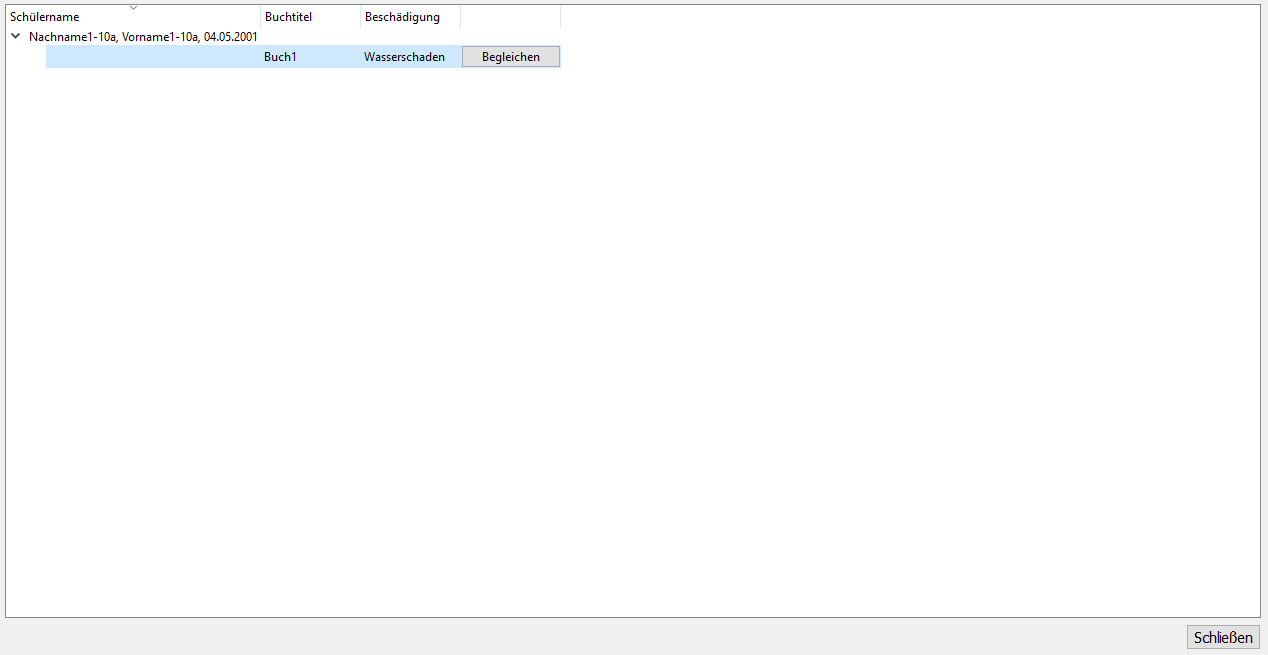
\includegraphics[width=0.70\textwidth]{figures/DamagesWidget.PNG}
	\caption{DamagesWidget}
	\label{fig:DamagesWidget}
\end{figure}

\textbf{StudentModel}\\
Das StudentModel enthält alle Informationen von Schülern. Es greift über die Datenbank-API auf die Informationen der Schülerdatenbank zu. Das Model ist von QAbstractTableModel abgeleitet, folgende Methoden sind implementiert:
\begin{description}
	\item[ ] StudentModel(StudentTable* stable, QObject* parent = 0)\\
	Konstruiert ein neues Objekt von StudentModel, das einen Pointer auf die StudentTable des Dataset erhält sowie optional einen parent.
  \item[ ] \~{}StudentModel()\\
	Zerstört das Objekt und löscht alle Daten aus dem Model.
	\item[ ] int rowCount(const QModelIndex \&parent) const\\
	Liefert die Anzahl der Schüler, also die Anzahl der Zeilen, zurück.
  \item[ ] int columnCount(const QModelIndex \&parent) const\\
	Gibt die Anzahl der Spalten (vier) zurück.
  \item[ ] QVariant data(const QModelIndex \&index, int role) const\\
	Es werden die einzelnen Informationen aus dem Model entsprechend dem index und der role herausgelesen.
  \item[ ] QVariant headerData(int section, Qt::Orientation orientation, int role) const\\
	Liefert die Headerinformationen pro Spalte: Name, Geburtsdatum und Klasse. Die vierte Spalte erhält keinen Header.
  \item[ ] void selectClass(QString className)\\
	Wählt eine Klasse aus. Dabei werden alle Schüler aus dem Model entfernt, die nicht in die gewählte Klasse gehören.
  \item[ ] void search(QString searchstring)\\
	Filtert gemäß des searchstring die Schüler aus dem Model (nicht passende Einträge werden aus dem Model entfernt).
	\item[ ] void deleteStudent(int row)\\
	Löscht den Schüler, der sich an der Stelle row befindet aus dem Model.
  \item[ ] void reset()\\
	Setzt das Model zurück.
  \item[ ] StudentTable::StudentRow* getStudent(QModelIndex index)\\
	Liefert die StudentRow aus dem Model an der Stelle index zurück, so dass die Zeile bearbeitet werden kann. Der Pointer darf nicht gelöscht werden!
  \item[ ] StudentTable::StudentRow* getStudent(int row)\\
	Gleiches Ergebnis wie bei getStudent(QModelIndex index) nur unter Angabe der Zeilennummer.
  \item[ ] void updateRow(int row)\\
	Die Zeile an der Position row wird aktualisiert. Diese Methode muss aufgerufen werden, wenn eine mit getStudent() erhaltene Zeile bearbeitet wurde. Das Model aktualisiert hierdurch die View.
  \item[ ] void addStudent(StudentTable::StudentRow* newRow)\\
	Ein neu angelegter Schüler wird in das Model eingefügt.
\end{description}
    
\textbf{StudentWidget}\\
Das StudentWidget zeigt mittels einer TableView die Einträge im StudentModel an, siehe Abbildung \ref{fig:StudentWidget}. Das Widget erlaubt es eine Klasse auszuwählen und damit alle Schüler dieser Klasse anzuzeigen. Zudem kann nach Schülern gefiltert werden. StudentWidget ist abgeleitet von QWidget. Die Methoden sind:
\begin{description}
	\item[ ] explicit StudentWidget(Dataset* set, UserPermissions permission, QWidget *parent = 0)\\
	Erzeugt ein StudentWidget-Objekt unter Übergabe eines Pointers auf das Dataset, UserPermissions und optional ein parent-Objekt.
  \item[ ] \~{}StudentWidget()\\
	Zerstört das Widget wieder und gibt den Speicherplatz frei.
	\item[ ] void closewidget()\\
	Das Signal wird ausgegeben, wenn das Widget aus dem parent-Element entfernt werden soll.	
\end{description}
\begin{figure}[htb]
	\centering
		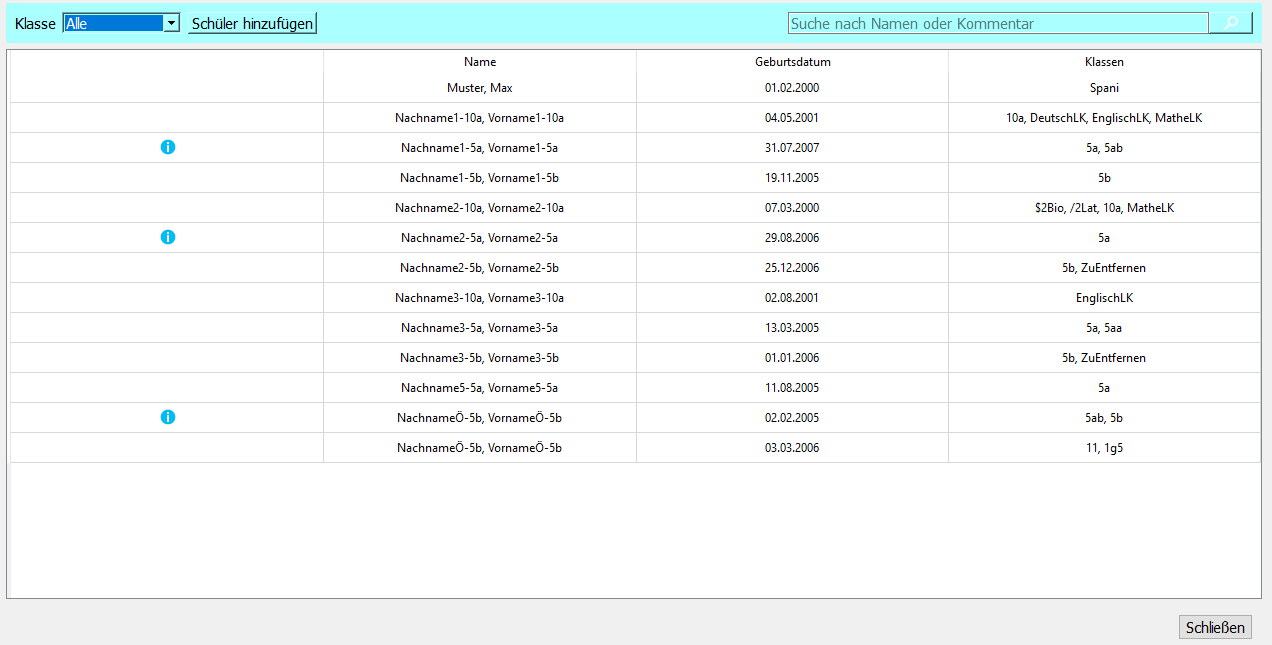
\includegraphics[width=0.60\textwidth]{figures/StudentWidget.PNG}
	\caption{StudentWidget}
	\label{fig:StudentWidget}
\end{figure}

\textbf{StudentMask}\\
Die StudentMask stellt eine Maske zur Bearbeitung bzw. Neuanlage eines Schülers dar. Die Eintragungen werden überwacht. Die Maske ist in Abbildung \ref{fig:StudentMask} dargestellt. Die Basisklasse ist QDialog, weitere Methoden sind:
\begin{description}
	\item[ ] explicit StudentMask(Dataset* set, QWidget* parent = 0)\\
	Erzeugt ein neues Objekt der StudentMask-Klasse. Es muss ein Pointer auf das Dataset und optional ein parent übergeben werden.
   \item[ ] \~{}StudentMask()\\
	Zerstört das Objekt.
   \item[ ] void selectStudent(StudentTable::StudentRow *row)\\
	 Überträgt den übergebenen Schüler (row) auf die Schülermaske, so dass diese row bearbeitet werden kann (die Änderungen werden beim Akzeptieren des Dialogs direkt in die row geschrieben).
   \item[ ] StudentTable::StudentRow* getNewStudent()\\
	Liefert den neu erzeugten Schüler zurück.
\end{description}
\begin{figure}[htb]
	\centering
		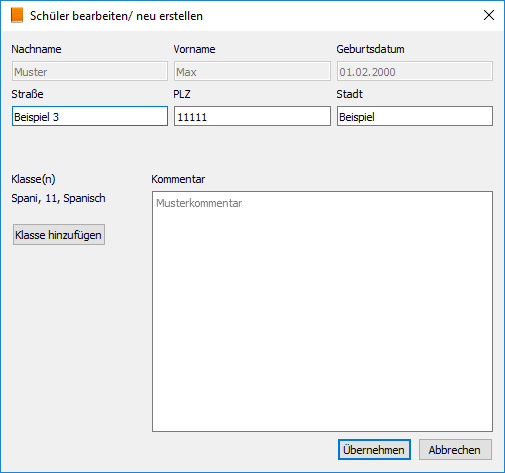
\includegraphics[width=0.60\textwidth]{figures/StudentMask.png}
	\caption{StudentMask}
	\label{fig:StudentMask}
\end{figure}

\textbf{AddClass}\\
AddClass stellt eine Maske zum Hinzufügen einer neuen Klasse dar. Die Eintragungen werden überwacht. 
\begin{description}
	\item[ ] explicit addclass(QWidget *parent = 0)\\
	Erzeugt ein neues Objekt der AddClass-Klasse. Es kann optional ein Pointer übergeben werden.
	\item[ ] ~addclass()\\
	Destruktor, zerstört das Objekt.
	\item[] ClassTable::ClassRow getNewClass()\\
	Liefert die neu erzeugte Klasse zurück.
\end{description}

\textbf{AddUserDialog}\\
AddUserDialog stellt den Dialog zum Hinzufügen eines neuen Benutzers bereit. Die Eintragungen werden überwacht. 
\begin{description}
	\item[] explicit adduserdialog(Dataset* set, QWidget *parent = 0)\\
	Erzeugt ein neues Objekt der AddUserDialog-Klasse. Es muss ein Pointer auf das verwendete Dataset und optional ein Parent übergeben werden.
	\item[] ~adduserdialog()\\
	Destruktor, zerstört das Objekt.
  	\item[] void selectUser(QString user, UserTable::UserRow* row)\\
	Füllt die gegebenen Benutzerdaten in den Benutzerdialog, um ihn zu bearbeiten. Benötigt den Namen des momentanen Benutzers, sowie die UserRow aus der UserTable der Datenbank.
  	\item[] UserTable::UserRow* getReturnUser()\\
	Liefert den neuen, bzw. den geänderten, Benutzer zurück.
\end{description}

\textbf{Dataset}\\
Das Dataset stellt die Daten dar, mit denen das Programm arbeitet und enthält daher die Daten, der Datenbank.
\begin{description}
	\item[] Dataset() \\
	Erzeugt eine neues Dataset Objekt.
	\item[] virtual ~Dataset() \\
	Destruktor, zerstört das Objekt.
  	\item[] UserTable mUserTable \\
  	Bildet die Benutzertabelle der Datenbank ab.
  	\item[] ClassTable mClassTable \\
  	Bildet die Klassentabelle der Datenbank ab.
  	\item[] StudentClassTable mStudentClassTable \\
  	Bildet die Student-Klassentabelle der Datenbank ab.
  	\item[] StudentTable mStudentTable \\
  	Bildet die Schülertabelle der Datenbank ab.
  	\item[] BookTable mBookTable \\
  	Bildet die Büchertabelle der Datenbank ab.
  	\item[] GiveBackTable mGiveBackTable \\
  	Bildet die Rückgabetabelle der Datenbank ab.
  	\item[] LendingTable mLendTable \\
  	Bildet die Ausleihtabelle der Datenbank ab.
\end{description}

\textbf{CheckBoxDelegate}\\
Erweitert ein TableWidget um eine klickbare Checkbox.
\begin{description}
	\item[ ] CheckBoxDelegate(QObject *parent = 0) \\
	Erzeugt ein neues CheckBoxDelegate Objekt. Optional kann ein Parent übergeben werden.
  	\item[ ] void paint(QPainter *painter, const QStyleOptionViewItem \&option, const QModelIndex \&index) const \\
	Rendert den Delegate für das übergebene Item, an Position index, mit den übergeben Optionen. Dafür wird ein painter, sowie Styleoptionen und der index übergeben. 
  	\item[ ] virtual bool editorEvent(QEvent *event, QAbstractItemModel *model, const QStyleOptionViewItem \&option, const QModelIndex \&index) \\
  	Wird aufgerufen wenn ein Event auf dem Item des Delegate aufgerufen wird. Es wird das auslösende Event, das Model, das QStyleOptionViewItem, sowie der Index des Items übergeben.
\end{description}

\textbf{LendDelegate}\\
Erweitert ein TableWidget um eine Checkbox, sowie einen Plus- und Minusbutton. Wird für die Ausleihfunktionalität benötigt. 
\begin{description}
	\item[ ] LendDelegate(QObject *parent = 0) \\
	Erzeugt ein neues LendDelegate Objekt. Optional kann ein Parent übergeben werden.
  	\item[ ] void paint(QPainter *painter, const QStyleOptionViewItem \&option, const QModelIndex \&index) const \\
	Rendert den Delegate für das übergebene Item, an Position index, mit den übergeben Optionen. Dafür wird ein painter, sowie Styleoptionen und der index übergeben.
  	\item[ ] virtual bool editorEvent(QEvent *event, QAbstractItemModel *model, const QStyleOptionViewItem \&option, const QModelIndex \&index) \\
  	Wird aufgerufen wenn ein Event auf dem Item des Delegate aufgerufen wird. Es wird das auslösende Event, das Model, das QStyleOptionViewItem, sowie der Index des Items übergeben.
\end{description}	

\textbf{SelectClass}\\
SelectClass stellt einen Dialog bereit um Klassen auszuwählen.
\begin{description}
	\item[ ] explicit SelectClass(Dataset* set, QList<ClassTable::ClassRow> classes, QWidget *parent = 0) \\
	Erzeugt ein neues SelectClass Objekt, dafür wird das Dataset, sowie eine Liste der Klassen und optional ein parent übergeben.
  	\item[ ] ~SelectClass() \\
	Destruktor, zerstört das Objekt.
  	\item[ ] QList<ClassTable::ClassRow> getSelectedClasses() \\
	Gibt eine Liste der im Dialog ausgewählten Klassen zurück.
	\item[ ] void close() \\
	Schließt den Dialog.
\end{description}

\textbf{UserManagementDialog}\\
UserManagementDialog stellt einen Dialog bereit, um die Benutzer der LibOrg Software zu verwalten.
\begin{description}
	\item[ ] explicit usermanagementdialog(Dataset *set, QString currentUser, QWidget *parent = 0) \\
	Erzeugt ein neues UserManagementDialog Objekt, hierfür wird das Dataset, sowie der Name des momentan angemeldeten Benutzers und, optional, ein Parent übergeben.
  	\item[ ] ~usermanagementdialog() \\
	Destruktor, zerstört das Objekt.
\end{description}

\textbf{UserModel (UserManagementDialog)}\\
UserModel stellt das Model bereit um den TableView im UserManagementDialog mit Daten zu füllen.
\begin{description}
	\item[ ] explicit UserModel(UserTable *table, QObject *parent = nullptr) \\
	Erzeugt einn neues UserModel Objekt, hierfür wird die Usertable und optional ein parent übergeben.
  	\item[ ] ~UserModel() \\
  	Destruktor, zerstört das Objekt.
	\item[ ] QVariant headerData(int section, Qt::Orientation orientation, int role = Qt::DisplayRole) const override \\
  	Gibt die Daten, die in den Header des Models gehören, zurück. Hierfür wird eine Section eine orientation und eine Role übergeben.
	\item[ ] int rowCount(const QModelIndex \&parent = QModelIndex()) const override \\
  	Gibt die Anzahl der Reihen zurück. Hierfür wird ein Index übergeben.
	\item[ ] int columnCount(const QModelIndex \&parent = QModelIndex()) const override \\
  	Gibt die Anzahl der Spalten zurück. Hierfür wird ein Index übergeben.
	\item[ ] QVariant data(const QModelIndex \&index, int role = Qt::DisplayRole) const override \\
  	Gibt die Daten für das Model zurück. Hierfür wird ein Index und eine Role übergeben.
	\item[ ] bool removeRows(int row, int count, const QModelIndex \&parent = QModelIndex()) override \\
	Löscht Reihen aus dem Model. Es wird die Startrow sowie die Anzahl der zu löschenden Reihen und ein Index übergeben.
	\item[ ] void reset() \\
  	Resettet das Model.
	\item[ ] void fillModel() \\
	Füllt das Model mit den zugehörigen Daten.
	\item[ ] UserTable::UserRow* getRow(int row) \\
  	Gibt die Reihe an der Stelle row zurück.
	\item[ ] void updateRow(UserTable::UserRow * updatedRow, int row) \\
  	Aktualisiert eine Reihe, hierfür wird der Index der Reihe sowie die neuen Daten, als UserRow, übergeben.
	\item[ ] void addRow(UserTable::UserRow * newRow) \\
	Fügt eine Reihe zum Model hinzu. Es wird die Reihe, welche hinzugefügt werden soll, übergeben.
\end{description}

\textbf{ClassModel}\\
Stellt das Model für einen TableView der Klassen bereit.
\begin{description}
	\item[ ] ClassModel(Dataset* set, QObject* parent = 0) \\
	Erzeugt ein neues ClassModel Objekt, hierfür wird das Dataset und optional ein parent übergeben.
  	\item[ ] ~ClassModel() \\	
	Destruktor, zerstört das Objekt.
  	\item[ ] int rowCount(const QModelIndex \&parent) const \\
	Gibt die Anzahl der Reihen zurück. Hierfür wird der Index des Models übergeben.
  	\item[ ] int columnCount(const QModelIndex \&parent) const \\
	Gibt die Anzahl der Spalten zurück, hierfür wird der Index des Models übergeben.
  	\item[ ] void initialize() \\
	Initialisiert das Model.
  	\item[ ] QVariant data(const QModelIndex \&index, int role) const \\
	Gibt die Daten des Models mit dem Index und der Role zurück.
 	\item[ ] bool setData(const QModelIndex \&index, const QVariant \&value, int role) \\
	Setzt die Daten des Models. Es wir der Index des Models sowie die Values und die Role übergeben.
 	\item[ ] QVariant headerData(int section, Qt::Orientation orientation, int role) const \\
	Gibt die Daten für den Header zurück. Hierür wird die Sektion, die Orietierung und die Role übergeben.
  	\item[ ] Qt::ItemFlags flags(const QModelIndex \&index) const \\
	Gibt die gesetzten Flags für ein Model mit dem Index index zurück.
  	\item[ ] QList<ClassTable::ClassRow> getSelectedClasses() \\
	Gibt die momentan ausgewählten Klassen zurück.
  	\item[ ] void addClass(ClassTable::ClassRow newClass) \\
	Fügt eine neue Klasse zum Model hinzu. Hierfür wird die neue Klasse übergeben.
  	\item[ ] void selectClasses(QList<ClassTable::ClassRow> toSelectClasses) \\
	Wird aufgerufen wenn bestimmte Klassen ausgewählt werden sollen. Hierfür werden die auszuwählenden Klassen übergeben.
  	\item[ ] void reset() \\
	Resettet das Model.
  	\item[ ] void fill() \\
	Füllt das Model mit Daten.
\end{description}

\textbf{BookingWidget}\\
Stelllt das Widget für die Bücher bereit.
\begin{description}
	\item[ ] explicit BookWidget(Dataset *set, QWidget *parent = 0) \\
	Erzeugt ein neues BookWidget Objekt, hierfür wird das Dataset und optional ein parent übergeben.
  	\item[ ] ~BookWidget() \\
	Destruktor, zerstört das Objekt.
	\item[ ] void closewidget() \\
	Beendet das Widget.
\end{description}

\textbf{SingleBookingDialog}\\
Stellt den Dialog für eine Ausleihe eines Buches an einen Schüler bereit.
\begin{description}	
    \item[ ] explicit ShortBookModel(StudentTable::StudentRow *row, StudentTable* stable, BookTable* btable, LendingTable* ltable, QWidget *parent = nullptr); \\
    Erzeugt ein neues ShortBookModel Objekt. Hierfür wird die Studentrow des Schülers, die Studenttable, die Booktable, die Lendingtable, sowie optional ein parent übergeben.
    \item[ ] ~ShortBookModel(); \\
    Destruktor, zerstört das Objekt.
    \item[ ] int rowCount(const QModelIndex \&parent = QModelIndex()) const override; \\
    Gibt die Anzahl der Reihen zurück, hierfür wird der Index des Models übergeben.
    \item[ ] int columnCount(const QModelIndex \&parent = QModelIndex()) const override; \\
    Gibt die Anzahl der Spalten zurück, hierfür wird der Index des Models übergeben.
    \item[ ] QVariant headerData(int section, Qt::Orientation orientation, int role) const; \\
    Gibt die Daten für den Header zurück. Es wird die Section, die Orientation, sowie die Role übergeben.
    \item[ ] QVariant data(const QModelIndex \&index, int role = Qt::DisplayRole) const override; \\
    Gibt die Daten für das Model zurück. Hierfür wird eine Index und eine Role übergeben.
    \item[ ] bool setData(const QModelIndex \&index, const QVariant \&value, int role); \\
    Setzt die Daten des Models. Es wir der Index des Models sowie die Values und die Role übergeben.
    \item[ ] Qt::ItemFlags flags(const QModelIndex \&index) const; \\
    Gibt die gesetzten Flags für ein Model mit dem Index index zurück.
    \item[ ] void select(option option); \\
    Wird aufgerufen, wenn sich die ausgewählte Option ändert. Hierfür wird die option übergeben.
    \item[ ] void setHolidayLending(bool value); \\
    Setzt eine Ausleihe auf Ferienausleihe. Es wird der zu setztende boolean Wert übergeben.
\end{description}

\textbf{StudentLendModel}\\
Stellt das Model für einen TableView, welcher die Ausleihen von Schülern darstellt, bereit.
\begin{description}
    \item[ ] StudentLendModel(StudentTable* stable, BookTable* btable, LendingTable* ltable, QFontMetrics font, QObject * parent = 0); \\
    Erzeugt ein neues StudentLendModel Objekt. Hierfür wird die Studenttable, die Booktable, die Lendingtable, ein Font und optional ein parent übergeben.
    \item[ ] ~StudentLendModel(); \\
    Destruktor, zerstört das Objekt.
    \item[ ] int rowCount(const QModelIndex \&parent) const; \\
    Gibt die Anzahl der Reihen zurück, hierfür wird der Index des Models übergeben.
    \item[ ] int columnCount(const QModelIndex \&parent) const; \\
    Gibt die Anzahl der Spalten zurück, hierfür wird der Index des Models übergeben.
    \item[ ] QVariant data(const QModelIndex \&index, int role) const; \\
    Gibt die Daten für das Model zurück. Hierfür wird ein Index und eine Role übergeben.
    \item[ ] QVariant headerData(int section, Qt::Orientation orientation, int role) const; \\
    Gibt die Daten für den Header zurück. Es wird die Section, die Orientation, sowie die Role übergeben.
    \item[ ] bool setData(const QModelIndex \&index, const QVariant \&value, int role); \\
    Setzt die Daten des Models. Es wir der Index des Models sowie die Values und die Role übergeben.
    \item[ ] Qt::ItemFlags flags(const QModelIndex \&index) const; \\
    Gibt die gesetzten Flags für ein Model mit dem Index index zurück.
    \item[ ] bool setHeaderData(int section, Qt::Orientation orientation, const QVariant \&value, int role); \\
    Setzt die Daten für den Header. Es wir die section, die orientation, der neue value sowie die role übergeben.
    \item[ ] void selectClass(QString classname, int grade, QString subject, BookOption mOption); \\
    Wird aufgerufen wenn eine neue Klasse ausgewählt wird, dabei wird der classname, die grade, das fach und eine bookoption übergeben.
    \item[ ] void selectBookOptions(BookOption option); \\
    Wird aufgerufen wenn sich die bookoption ändert. Hierfür wird die neue Bookoption übergeben.
    \item[ ] void reset(); \\
    Resettet das Model.
    \item[ ] void setDialogParent(QWidget *parent); \\
    Setzt den parent des Dialogs auf den übergebenen parent.
   	\item[ ] void searchInBooks(QString searchString, BookOption mOption); \\
   	Führt eine Suche in den Büchern des Models durch. Hierfür wird der searchstring, sowie die momentane bookoption übergeben.
    \item[ ] StudentTable::StudentRow* getStudent(QModelIndex index); \\
   	Gibt den Schüler an der Stelle index zurück.
\end{description}

\textbf{OpenLendings}\\
Stellt den Dialog, um die Ausleihen eines Schülers anzuzeigen, bereit.
\begin{description}
	\item[ ] LendBooksModel(Dataset *set, QObject* parent); \\
	Erzeugt ein neues LendBookModel Objekt, hierfür wird das Dataset und optional ein parent übergeben.
    \item[ ] ~LendBooksModel(); \\
    Destruktor, zerstört das Objekt.
    \item[ ] void selectOption(QString option); \\
    Wird aufgerufen, wenn sich die Bookoption ändert, es wird die neue Option als String übergeben.
    \item[ ] StudentTable::StudentRow* getStudent(QModelIndex index); \\
    Gibt den Schüler an der Stelle index zurück.
    \item[ ] void updateRow(QModelIndex index); \\
    Aktualisiert die Reihe an der Stelle index.
    \item[ ] int rowCount(const QModelIndex \&parent) const; \\
    Gibt die Anzahl der Reihen zurück, hierfür wird der Index des Models übergeben.
    \item[ ] int columnCount(const QModelIndex \&parent) const; \\
    Gibt die Anzahl der Spalten zurück, hierfür wird der Index des Models übergeben.
    \item[ ] QVariant data(const QModelIndex \&index, int role) const; \\
    Gibt die Daten für das Model zurück. Hierfür wird eine Index und eine Role übergeben.
    \item[ ] QVariant headerData(int section, Qt::Orientation orientation, int role) const; \\
    Gibt die Daten für den Header zurück. Es wird die Section, die Orientation, sowie die Role übergeben.
    \item[ ] bool setData(const QModelIndex \&index, const QVariant \&value, int role); \\
    Setzt die Daten für das Model. Es wird der index, das zu setzende value und die role übergeben.
    \item[ ] Qt::ItemFlags flags(const QModelIndex \&index) const; \\
	Gibt die gesetzten Flags für ein Model mit dem Index index zurück.
\end{description}


\textbf{MainWindow}  \\
Das MainWindow, siehe Abbildung \ref{fig:MainWindow}, stellt das Hauptfenster bzw. die Hauptanwendung dar. Von ihm aus können alle Funktionen der Software ausgeführt werden. Aus diesem Grund werden nicht die öffentlichen Methoden sondern alle anderen Methoden der MainWindow-Klasse vorgestellt:
\begin{description}
	\item[ ] Slot: void rider\_settings\_triggered()\\
	Öffnet den Dialog für die Einstellungen, dabei wird die Klasse SettingsDialog verwendet.
  \item[ ] Slot: void rider\_about\_triggered()\\
	Es wird ein Objekt von AboutDialog angelegt und angezeigt.
  \item[ ] Slot: void rider\_import\_triggered()\\
	Öffnet den Dialog zum Import der ASV- und WinQD-Dateien.
  \item[ ] Slot: void rider\_changeuser\_triggered()\\
	Der Slot wird aufgerufen, wenn der aktuelle Benutzer gewechselt werden soll. Es wird der LoginDialog aufgerufen und bei Eingabe eines neuen Benutzers samt Passwort das Fenster mit den aktuellen Berechtigungen versorgt.
  \item[ ] Slot: void rider\_3rd\_party\_software\_triggered()\\
	Dieser Slot zeigt den Lizenzdialog der Klasse Licenceplugin an.
  \item[ ] Slot: void rider\_lend\_and\_giveback\_triggered()\\
	Platziert ein BookingWidget-Objekt in das vorgesehene leere Widget-Element und zeigt es an. Befand sich vorab ein anderes Objekt in diesem Widget-Element, so wird dieses entfernt.
  \item[ ] Slot: void rider\_books\_triggered()\\
	Leert das Widget-Element und fügt das BookWidget in es ein.
  \item[ ] Slot: void rider\_students\_triggered()\\
	Legt das StudentsWidget im Widget-Element ab, nachdem dieses geleert wurde.
  \item[ ] Slot: void clearWidget()\\
	Dieser Slot wird vor jedem Einfügen eines neuen Widgets in das Widget-Element vom entsprechenden Slot aufgerufen. Zudem wird der Slot aufgerufen, wenn ein Widget im Widget-Element das Signal closewidget() emittiert. 
  \item[ ] Slot: void rider\_restoration\_triggered()\\
	Öffnet einen Dialog zur Wiederherstellung. Hierzu wird die Klasse DatabaseRestoration benutzt.
  \item[ ] Slot: void rider\_usermanagement\_triggerd()\\
	Erlaubt das Hinzufügen, Bearbeiten und Entfernen von Benutzern durch Verwendung der Klasse usermanagementdialog.
  \item[ ] Slot: void rider\_open\_lendings\_triggered()\\
	Leert das Widget-Element und legt ein OpenLendings-Widget darin ab.
  \item[ ] Slot: void rider\_damages\_triggered()\\
	Platziert ein DamagesWidget in das zuvor geleerte Widget-Element. Mit diesem Widget sind alle beschädigten Bücher ersichtlich.
	\item[ ] void closeEvent(QCloseEvent *event)\\
	Der Handler wird aufgerufen, bevor das Fenster geschlossen wird. Der Benutzer wird gefragt, ob der das Programm wirklich beenden will. Wenn nicht wird das Schließen des Fensters abgebrochen.
  \item[ ] void paintEvent(QPaintEvent *event)\\
  Dieses Event ist überladen worden, um herauszufinden, wenn ein Fenster das erste Mal angezeigt wird. Sie ruft window\_loaded() auf.
	\item[ ] void initUiWithPermissions (UserPermissions permissions)\\
	Aktiviert die Funktionen des Fensters gemäß den übergebenen permissions.
	\item[ ] void window\_loaded()\\
	Wird aufgerufen, nachdem das Fenster angezeigt wird. Es wird ein Backup durchgeführt, falls in der Konfiguration zu dieser Zeit ein Backup eingestellt ist. Danach erscheint der Login-Dialog. Wird kein gültiges Benutzer-Passwort-Paar eingetragen, bleiben alle Funktionen der Anwendung (außer Benutzer wechseln) deaktiviert. Anderenfalls wird das Fenster entsprechend den Berechtigungen aktiviert.
	\item[ ] void styleWindow()\\
	Diese Methode wird vom Konstruktor aufgerufen und passt das Hauptfenster entsprechend der Konfigurationsdatei an.
\end{description}
\begin{figure}[htb]
	\centering
		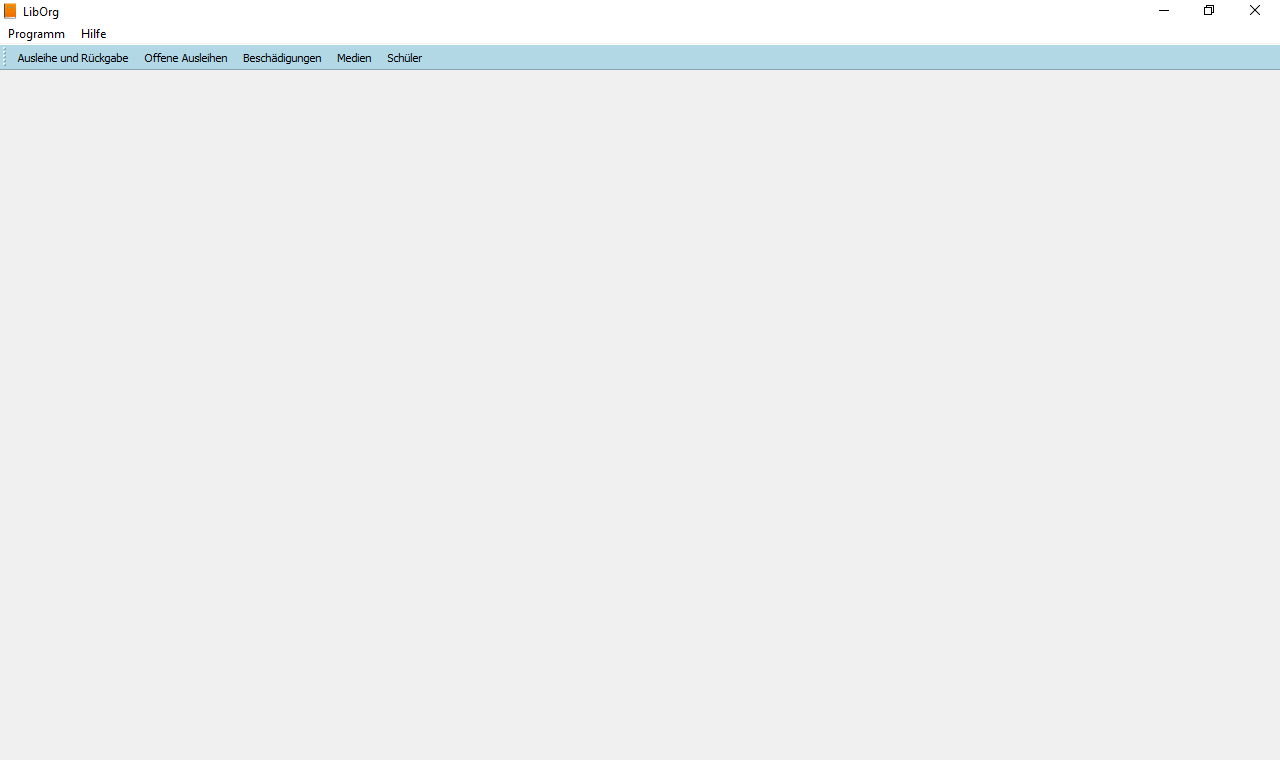
\includegraphics[width=0.70\textwidth]{figures/MainWindow.png}
	\caption{Hauptfenster}
	\label{fig:MainWindow}
\end{figure}
